\section {Estudo de Caso}

Visando a validação da solução apresentada na Seção \ref{sec:solucao}, foram consultadas as instituições citadas pelo Acórdão no 2314/2013 \cite{TCU:2013}. Dentre elas, o Instituto do Patrimônio Histórico e Artístico Nacional (IPHAN) que é autarquia da administração pública federal responsável pela gestão de diversos processos de preservação do patrimônio cultural, permitiu o acesso ao processo, documentos e o código-fonte Sistema Integrado de Gestão do Conhecimento (SICG), um dos primeiros softwares desenvolvidos sob um contrato de terceirização de serviços com a utilização de metodologias ágeis.

O Sistema Integrado de Gestão do Conhecimento (SICG) teve como objetivo automatizar o processo de trabalho decorrente da metodologia de inventário, cadastro, normatização, fiscalização, planejamento e análise e gestão do patrimônio material. Esta solução de software foi construída na linguagem Java com a utilização de\textit{frameworks} como VRaptor e Hibernate, durante 24 \textit{releases} mensais. Possui um total 39.790 linhas de código distribuídas em 914 classes.

\subsection{Protocolo do Estudo de Caso}
Seguindo a metodologia proposta por Wohlin \cite{wohlin2012experimentation}, foi construído um protocolo de estudo de caso que foi baseado em Brereton \cite{brereton2008using} quanto aos aspectos gerais e Yin \cite{yin2011applications} com relação as ameaças à validade do estudo. 

O objeto do estudo de caso é o ambiente de DWing projetado e implementado conforme apresentado na seção 3. A fonte de coleta dos dados, foi o código fonte do SICG. A partir do objetivo da pesquisa, foram elaborados objetivos específicos do estudo de caso utilizando o GQM \cite{Basili96b}. Nesta abordagem cada objetivo específico derivou uma série de questões específicas que são respondidas com métricas específicas, tal como se mostra na Tabela \ref{tbl:obj}

\begin{table}[ht]
\centering
\caption{Objetivos Específicos do Estudo de Caso}
\addtolength{\belowcaptionskip}{6pt}
\input{tabelas/objetivos.ltx}
\label{tbl:obj} 
\end{table}
\FloatBarrier


Com relação as ameaças citadas por Yin, a ameça à avalidade de de construção foi mitigada com utilização da abordagem GQM, uma vez que, esta estratégia estabelece uma lógica que une as proposições às métricas utilizadas no estudo. A validade interna é obtida quando se consegue observar as relações causais e todos os elementos que as compõem. No presente estudo de caso, pela própria definição de $T_r$, há uma relação diretamente proporcional à $C_e$, e inversamente proporcional à $C_l$, estabelecendo as relações causais. Quanto a validade externa, destaca-se que a utilização de um estudo de caso não é suficiente para generalizar os resultados deles obtidos, sendo necessário a utilização de estudo em múltiplos casos, a fim de aumentar o poder de generalização \cite{yin2011applications}. Com relação a confiabilidade, a partir da documentação da implementação do ambiente de \textit{Data Warehousing} conjuntamente com o protocolo de estudo de caso e as bases de dados das métricas de código-fonte, garante-se a repetição do estudo de caso e por conseguinte a confiabilidade.

\subsection{Execução e Resultados do Estudo de Caso}
\label{sec:resultados}
Para analisar os cenários de limpeza de código-fonte, foram extraídas as métricas de código-fonte de cada classe e analisadas conforme a Tabela \ref{tab:cenarios}. Para cada \textit{release}, foram identificados, conforme a Figura \ref{fig:cenarios-release}, os cenários de limpeza de código-fonte. Para se mostrar maior nível de detalhes dos cenários de limpeza de código-fonte, realizou-se uma consulta OLAP de \textit{Drill-Down}, que tem objetivo de expor mais detalhes na visualização dos dados \cite{Kimball2002}, sobre o modelo dimensional do \textit{data warehouse}. 


\begin{figure}[ht!]
\centering
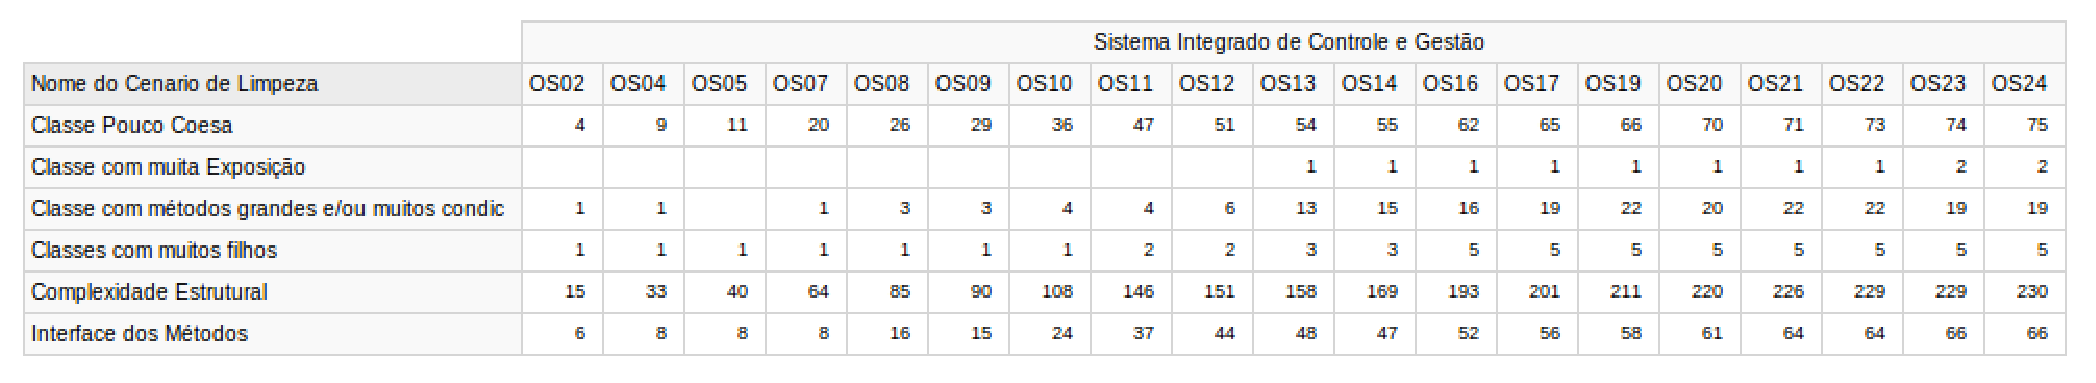
\includegraphics[keepaspectratio=true,scale=0.43]{figuras/total-cenario-tipo.eps}
\caption{Total de Cenários de Limpeza de Código-Fonte identificados por cenário e \textit{Release}}
\label{fig:cenarios-release}
\end{figure}
\FloatBarrier

A fim de se obter o número total de cenários de limpeza por cada uma das releases de software analisadas, como se observa na Figura \ref{fig:cenarios-total}, foi realizada uma consulta OLAP de \textit{Drill-Up}, que tem o objetivo de agregar o nível de visualização dos dados \cite{Kimball2002}, sobre os dados obtidos na Figura \ref{fig:cenarios-release}.

\begin{figure}[ht!]
\centering
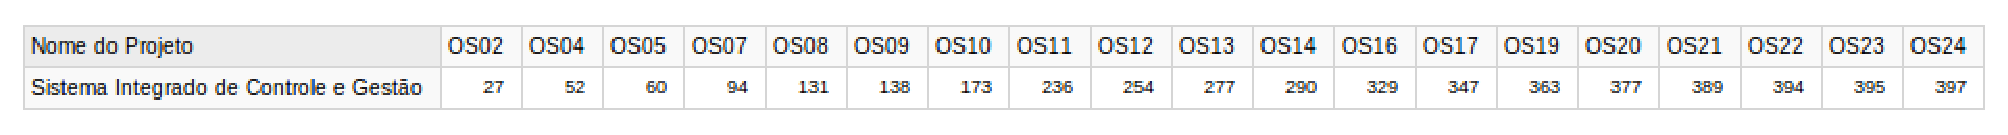
\includegraphics[keepaspectratio=true,scale=0.45]{figuras/total-cenarios-release.eps}
\caption{Total de Cenários de Limpeza de Código-Fonte por Release}
\label{fig:cenarios-total}
\end{figure}
\FloatBarrier

Conforme é possível observar nas Figuras \ref{fig:cenarios-release} e \ref{fig:cenarios-total}, foram detectados mais cenários de limpeza de código-fonte dos tipos \textbf{Complexidade Estrutural}, que corresponde entre 55\% a 68\% da quantidade total de cenários identificados; \textbf{Classe Pouco Coesa} e \textbf{Interface dos Métodos} respectivamente. Os três Cenários de Limpeza com menor número de incidências foram \textbf{Classe com Muita Exposição}, \textbf{Classe com Muitos Filhos} e \textbf{Classe com Métodos Muito Grande e/ou com muitos condicionais}.

Considerando que é importante conhecer as classes com maior incidência de problemas com relação limpeza de código-fonte, foram identificadas, como se mostra na Figura \ref{fig:worst-10-cenarios}, as 10 classes que apresentaram a maior quantidade de cenários de limpeza de código-fonte. Para se obter a informação desta consulta foram necessárias uma consulta OLAP de \textit{Drill Down} sobre algumas dimensões e outra de \textit{Slice and Dice}, que tem o objetivo de selecionar os dados, sobre o resultado a consulta de \textit{Drill-Down}.    

\begin{figure}[ht!]
\centering
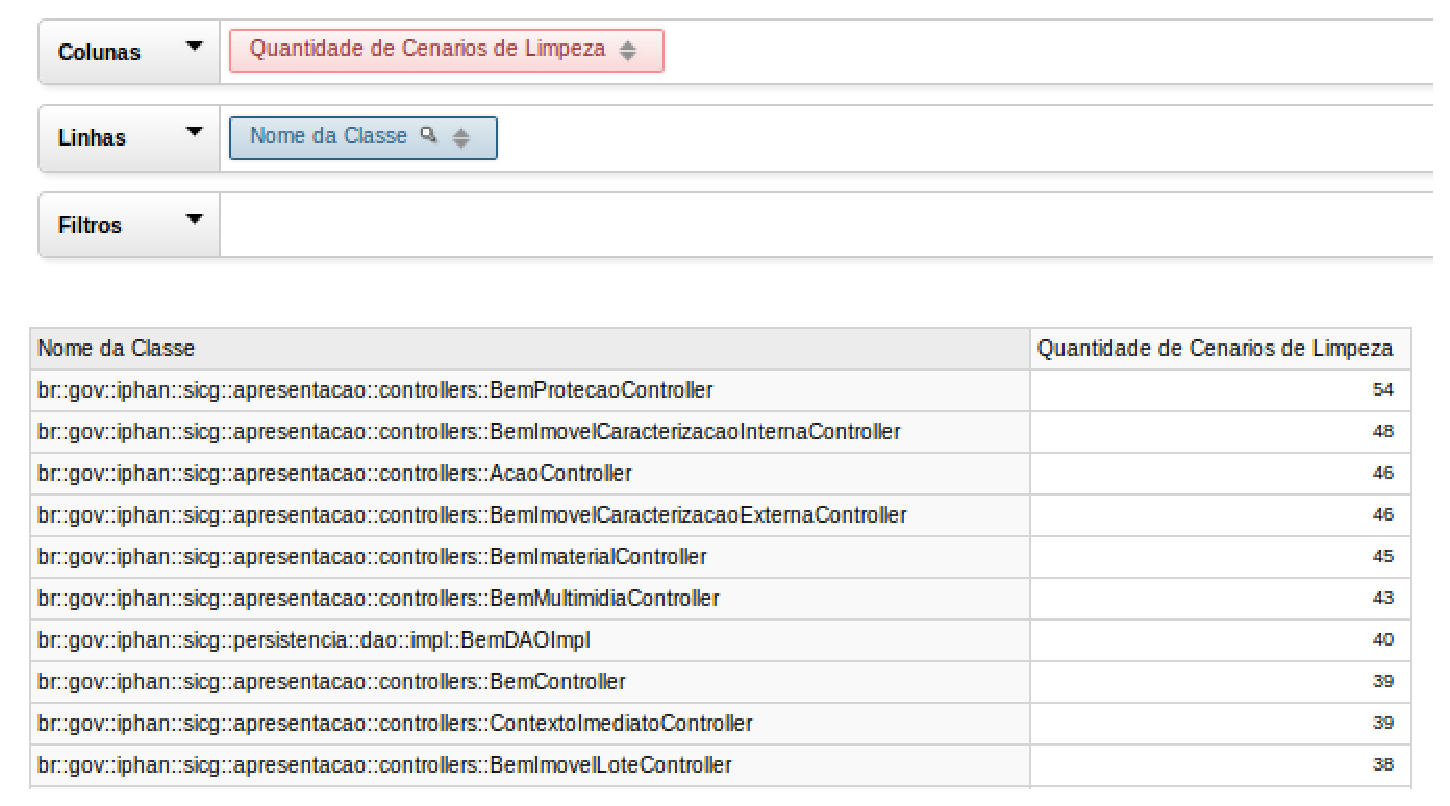
\includegraphics[keepaspectratio=true,scale=0.55]{figuras/10-best.eps}
\caption{As 10 classes com maior número identificado de Cénarios de Limpeza}
\label{fig:worst-10-cenarios}
\end{figure}
\FloatBarrier

Com a quantidade de classes e o total de cenários de limpeza de código-fonte, foi possível calcular a Taxa de Aproveitamento de Oportunidade de Melhoria de Código-Fonte por cada release do software conforme se mostra na Figura \ref{fig:taxa-cenarios}.

\begin{figure}[H]
\centering
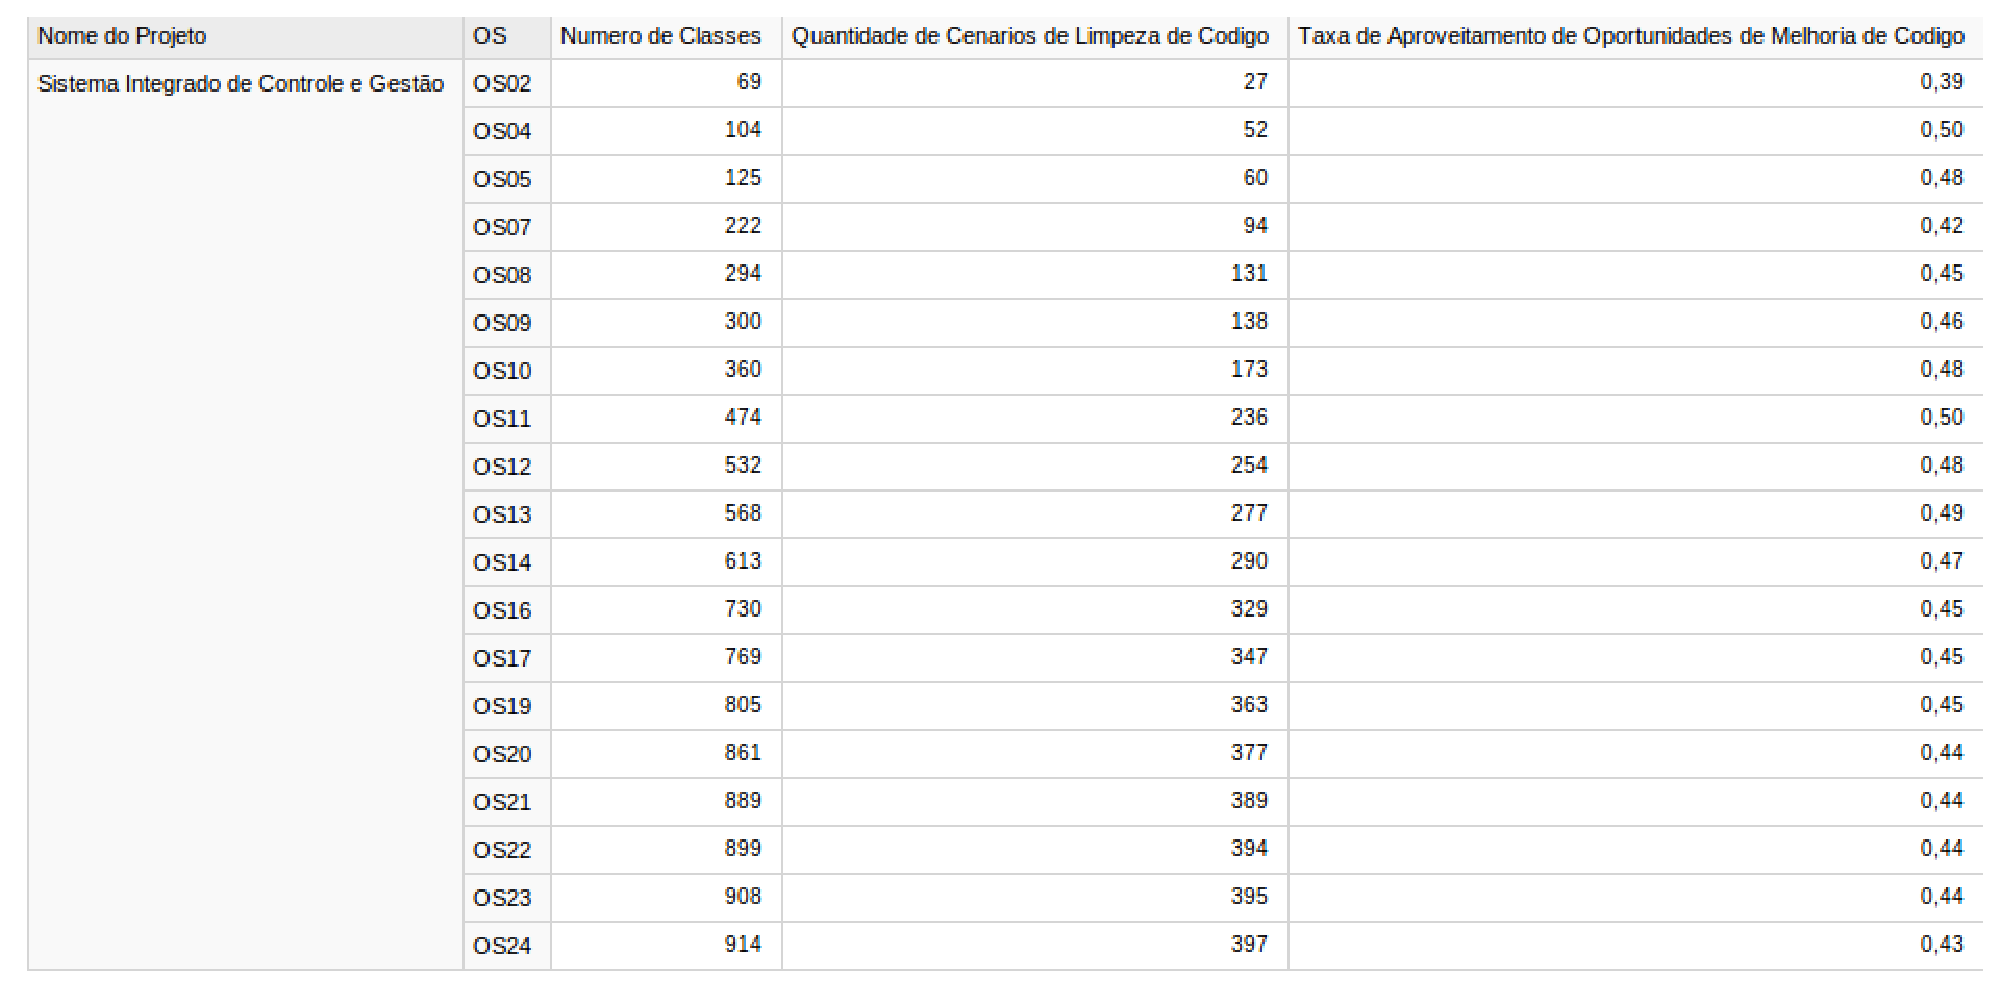
\includegraphics[keepaspectratio=true,scale=0.38]{figuras/taxa-parcial.eps}
\caption{Taxa de Aproveitamento de Oportunidades de Melhoria de Código-Fonte}
\label{fig:taxa-cenarios}
\end{figure}
\FloatBarrier


Considerando o comportamento da Taxa de Aproveitamento de Oportunidade de Melhoria de Código-Fonte apresentado na Figura \ref{fig:taxa-cenarios}, verifica-se que o valor variou entre 0,4 a 0.5 no decorrer do projeto. Este fato pode indicar que o projeto cresceu em uma taxa muito maior que a quantidade de cenários de limpeza, logo verificando-se assim uma estabilidade na complexidade do projeto.

